\documentclass[12pt, a4paper]{article}

\usepackage[utf8]{inputenc}
\usepackage[french]{babel}
\usepackage{graphicx}
\usepackage{color}
\usepackage{hyperref}

\usepackage[]{fullpage}

\graphicspath{{graphs/}}
\hypersetup{
    colorlinks,
    citecolor=black,
    filecolor=black,
    linkcolor=black,
    urlcolor=black
}

\title{Implantations efficaces de calculs sur les polynômes à une variable : FFT}
\author{}
\date{7 Avril 2022}

\begin{document}
\maketitle
\tableofcontents
\newpage

\section*{Introduction}
\addcontentsline{toc}{section}{Introduction}
Dans le cadre de l'UE LU2IN013, nous avons réalisé un projet sur l'optimisation de calculs sur les polynômes à une variable. Le but final de ce projet est la multiplication de deux polynômes le plus efficacement possible.\\
Pour ce faire, nous nous intéressons à plusieurs type d'algorithmes pour la multiplication, notamment : l'algorithme naïf, de Karatsuba et FFT.\\
Nous avons tout d'abord commencé avec Python mais nous avions besoin d'un langage bas niveau pour plus de rapidité d'où le fait qu'on a rapidement changé pour le langage C.\\


\section{Algorithme Naïf et de Karatsuba}
\subsection{Implémentation}
Pour commencer, nous avons réalisé un algorithme simple de multiplication (l'algorithme naïf) qui consiste à multiplier terme à terme chaque coefficients des polynômes. Par sa simplicité, cette algorithme nous permettait de vérifier les résultats de nos futurs algorithme plus performants.\\
Après cela, grâce aux différents ouvrages 
%mettre un aterix et mettre qq sources ?% 
trouvés sur internet, nous avons implémenté l'algorithme de Karatsuba 
\subsection{Comparaison - Naïf/Karatsuba}

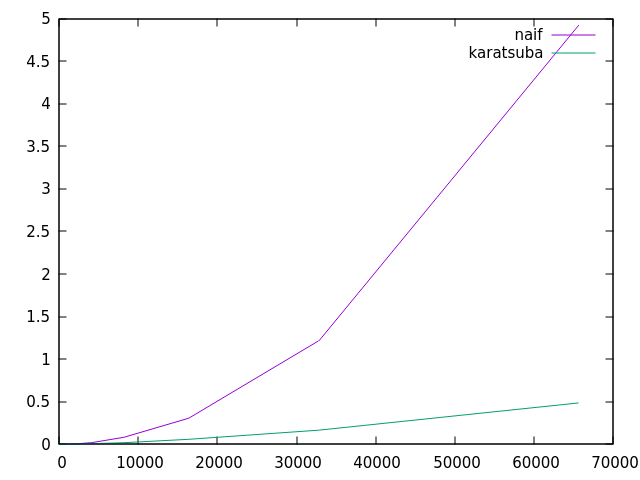
\includegraphics[scale=1]{naif_kara}\\


\section{Fast Fourier Transform (FFT)}
\subsection{Fonctionnement}
\subsection{Évalution d'un polynôme en un point}
\subsubsection{Implémentation}
\subsubsection{Tests de temps}

l'équation dans la phrase $e^{i\pi}+1 = 0$\\
l'équation au milieu numerotée
\begin{equation}
E=mc^2
\end{equation}
l'equation au mileu non numerotée
\[ E=mc^2 \]

Ceci est une liste :
\begin{enumerate}
  \item premier element
  \item deuxieme element
\end{enumerate}

\end{document}
